We have used two Bayesian implementations to cross check our results. The first Bayesian calculation is using numeric integration assuming a flat prior to derive a one sided $95\%$ credible interval and the second one is using Markov Chain Monte Carlo sampling which is based on the Metropolis-Hastings algorithm~\cite{MCMC}. 


For the centrality integrated bin (0 -100\%) the computed upper limit for the single ratio of 3S/1S using the Feldman-Cousins method 
is $R_{3}=0.0695 \pm 0.0004$ which can be seen from \fig{fig:FC_results}. 
when the observed $CL_s$ (red dots) crosses the horizontal threshold (red line). 
In~\fig{fig:FC_Centrality} 
we present the upper limits for all the centrality bins as a function of the number of participants. The two lowest values for the upper limits were found in the centrality bins where we had negative yields from the fitted results. These upper limits are indeed positive as expected. 
Figure~\ref{fig:limits_xchecks} %%Figure 35 %FIXME!!!!!! 
shows cross checks using different implementations.  
Figs.~\ref{fig:CLs_0100} and~\ref{fig:Asmp_0100} %a) and b) %FIXME!!!!!! 
use $CL_{s}$ and its asymptotic  approximation, and 
Figs.~\ref{fig:bayesian_post_0100},~\ref{fig:bayesian_mcmc_0100} %c) and d) %FIXME!!!!!! 
use Bayesian numeric integration and Markov Chain Montecarlo, respectively. Notice that all results are consistent within uncertainties.  
Finally, %FIXME... where???
in \fig{fig:bayesian},  
 we show Bayesian results in the (30-40\%) centrality bin where we found negative ratios.
%
%The results for the various centrality bins are shown in Tables~\ref{tab:upperlimits} and~\ref{tab:credible_intervals}. 
The upper limits found for the different centrality bins are tabulated in Tables~\ref{tab:upperlimits} and~\ref{tab:credible_intervals}. 

%FIXME: PLOTS ARE NOT REFERENCED/EXPLAINED IN THE TEXT

\begin{figure}[hbtp]
  \begin{center}
    %\subfigure[Upper limits for all centrality bins.]
{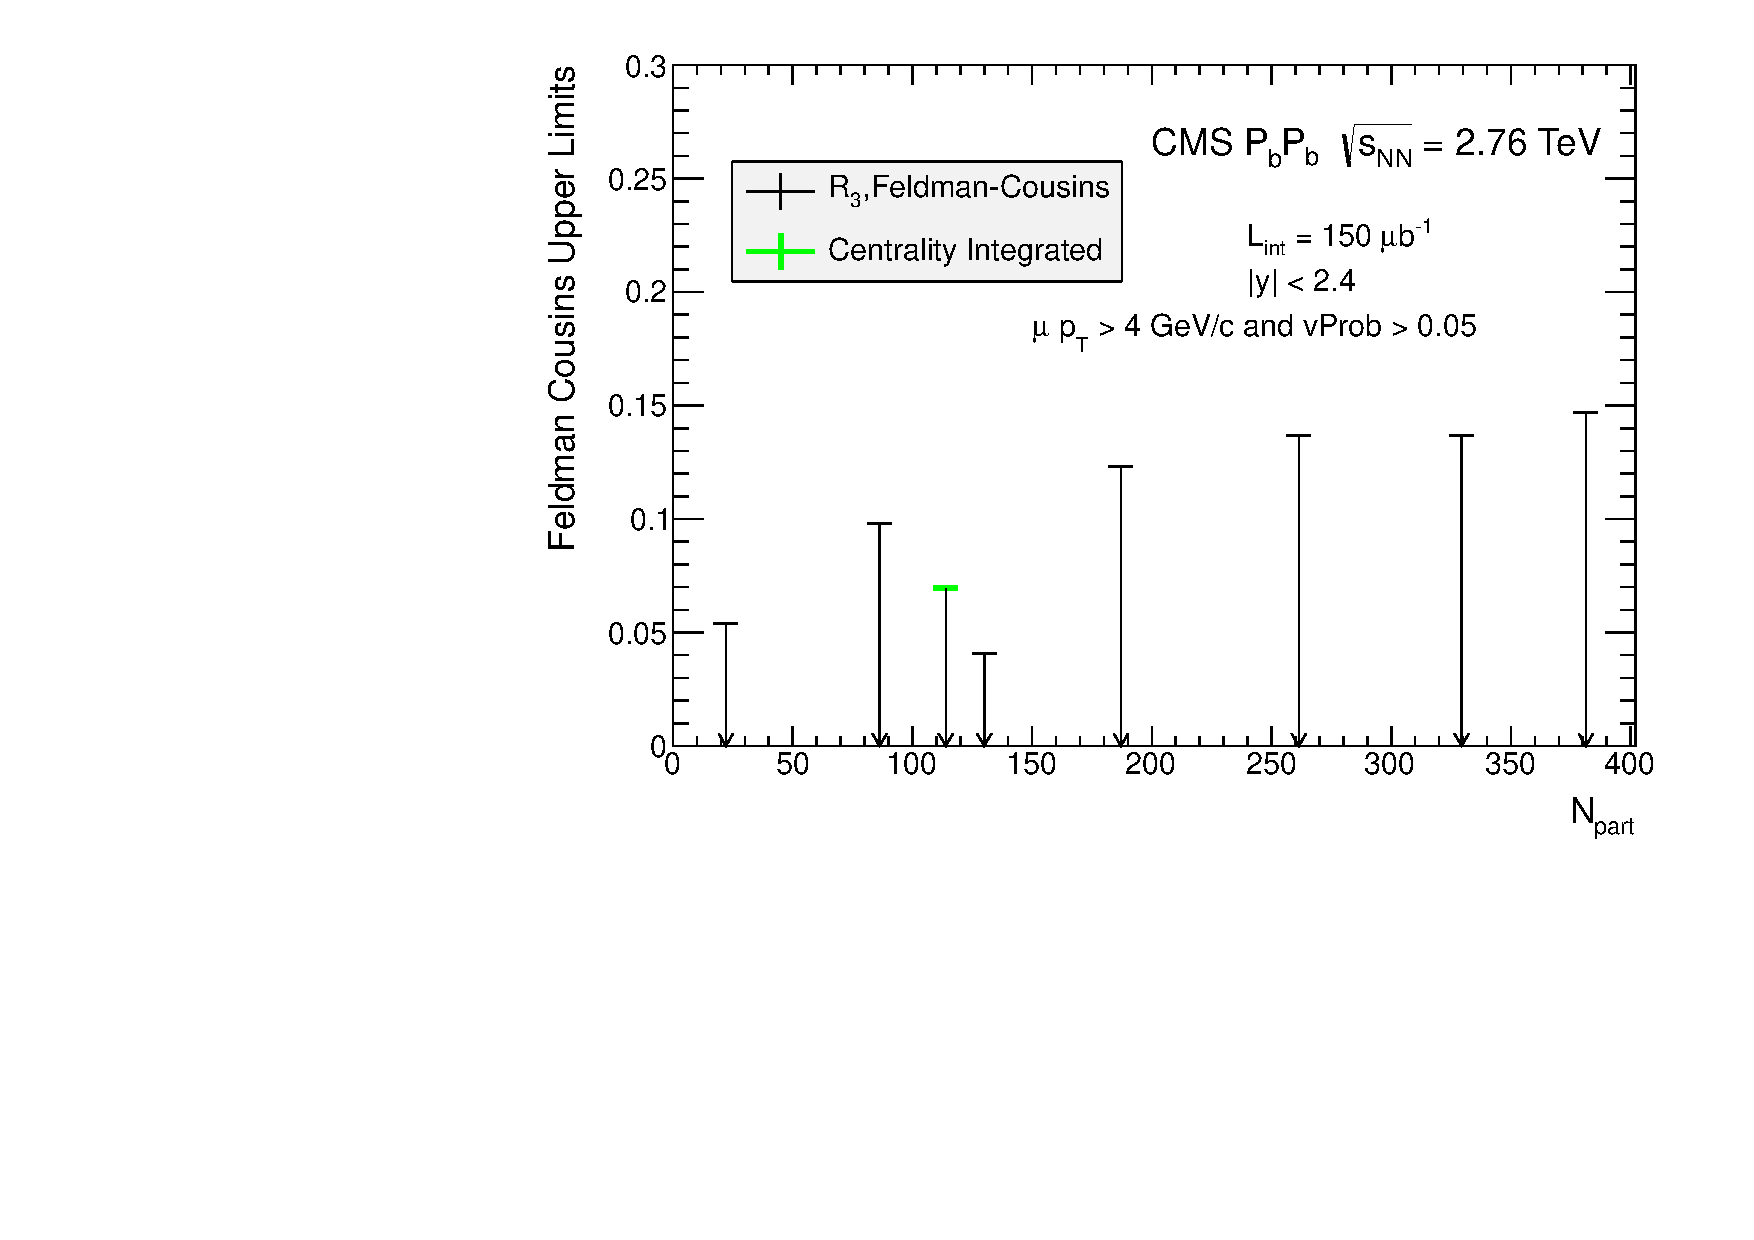
\includegraphics[angle=0,width=0.45\textwidth]{figures/limits/FC_Centrality}\label{fig:FC_Centrality}}
   \caption{Upper limit results using the Feldman-Cousins method on $R_3$ in \PbPb, evaluated for the different centrality bins. \emph{(Note: being updated)}
}
    \label{fig:FC_Centrality}
  \end{center}
\end{figure}


\begin{figure}[hbtp]
  \begin{center}
    \subfigure[Observed CLs crosses the 0.05 red line]{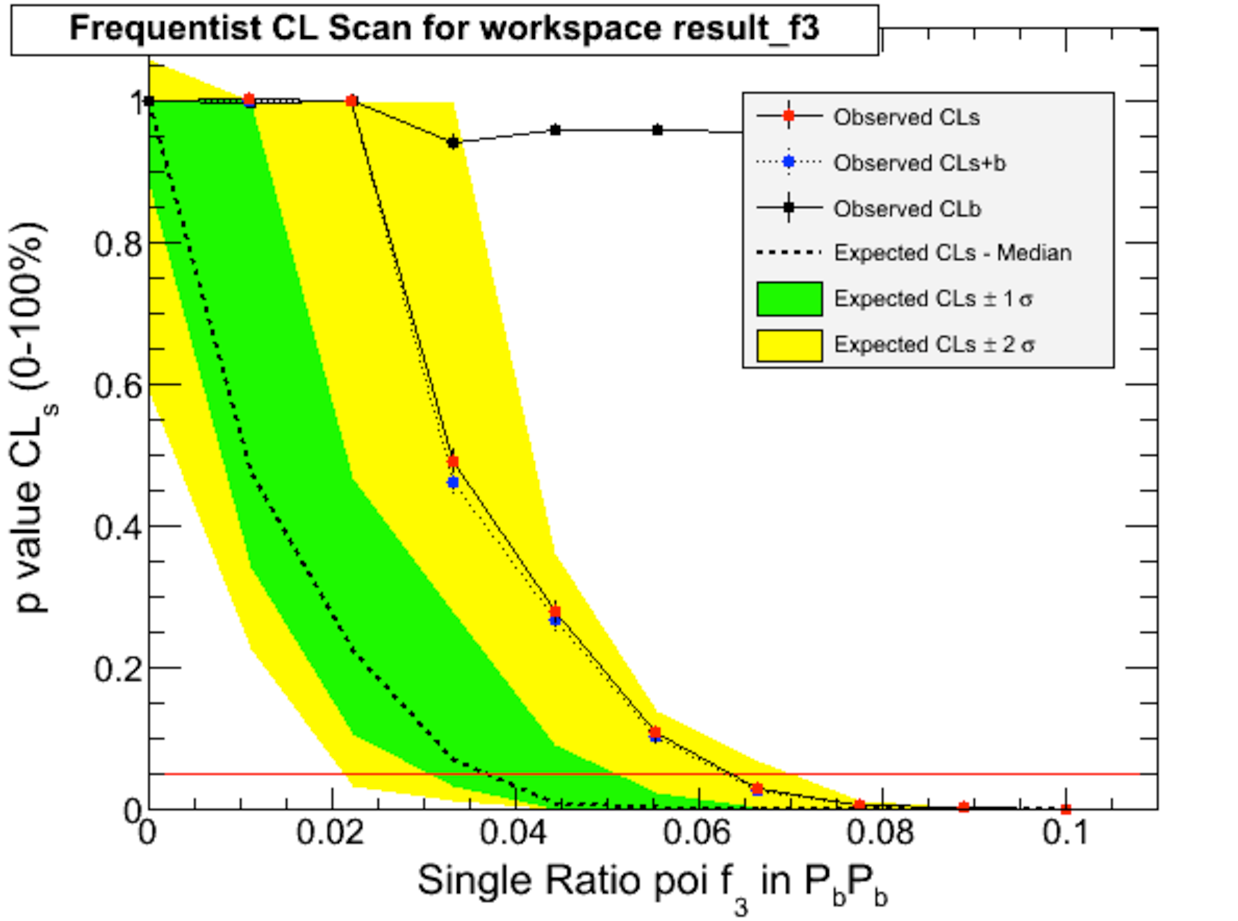
\includegraphics[angle=0,width=0.5\textwidth]{figures/limits/Cls_0100}\label{fig:CLs_0100}}
    \subfigure[Asymptotic approach using Asimov test statistics]{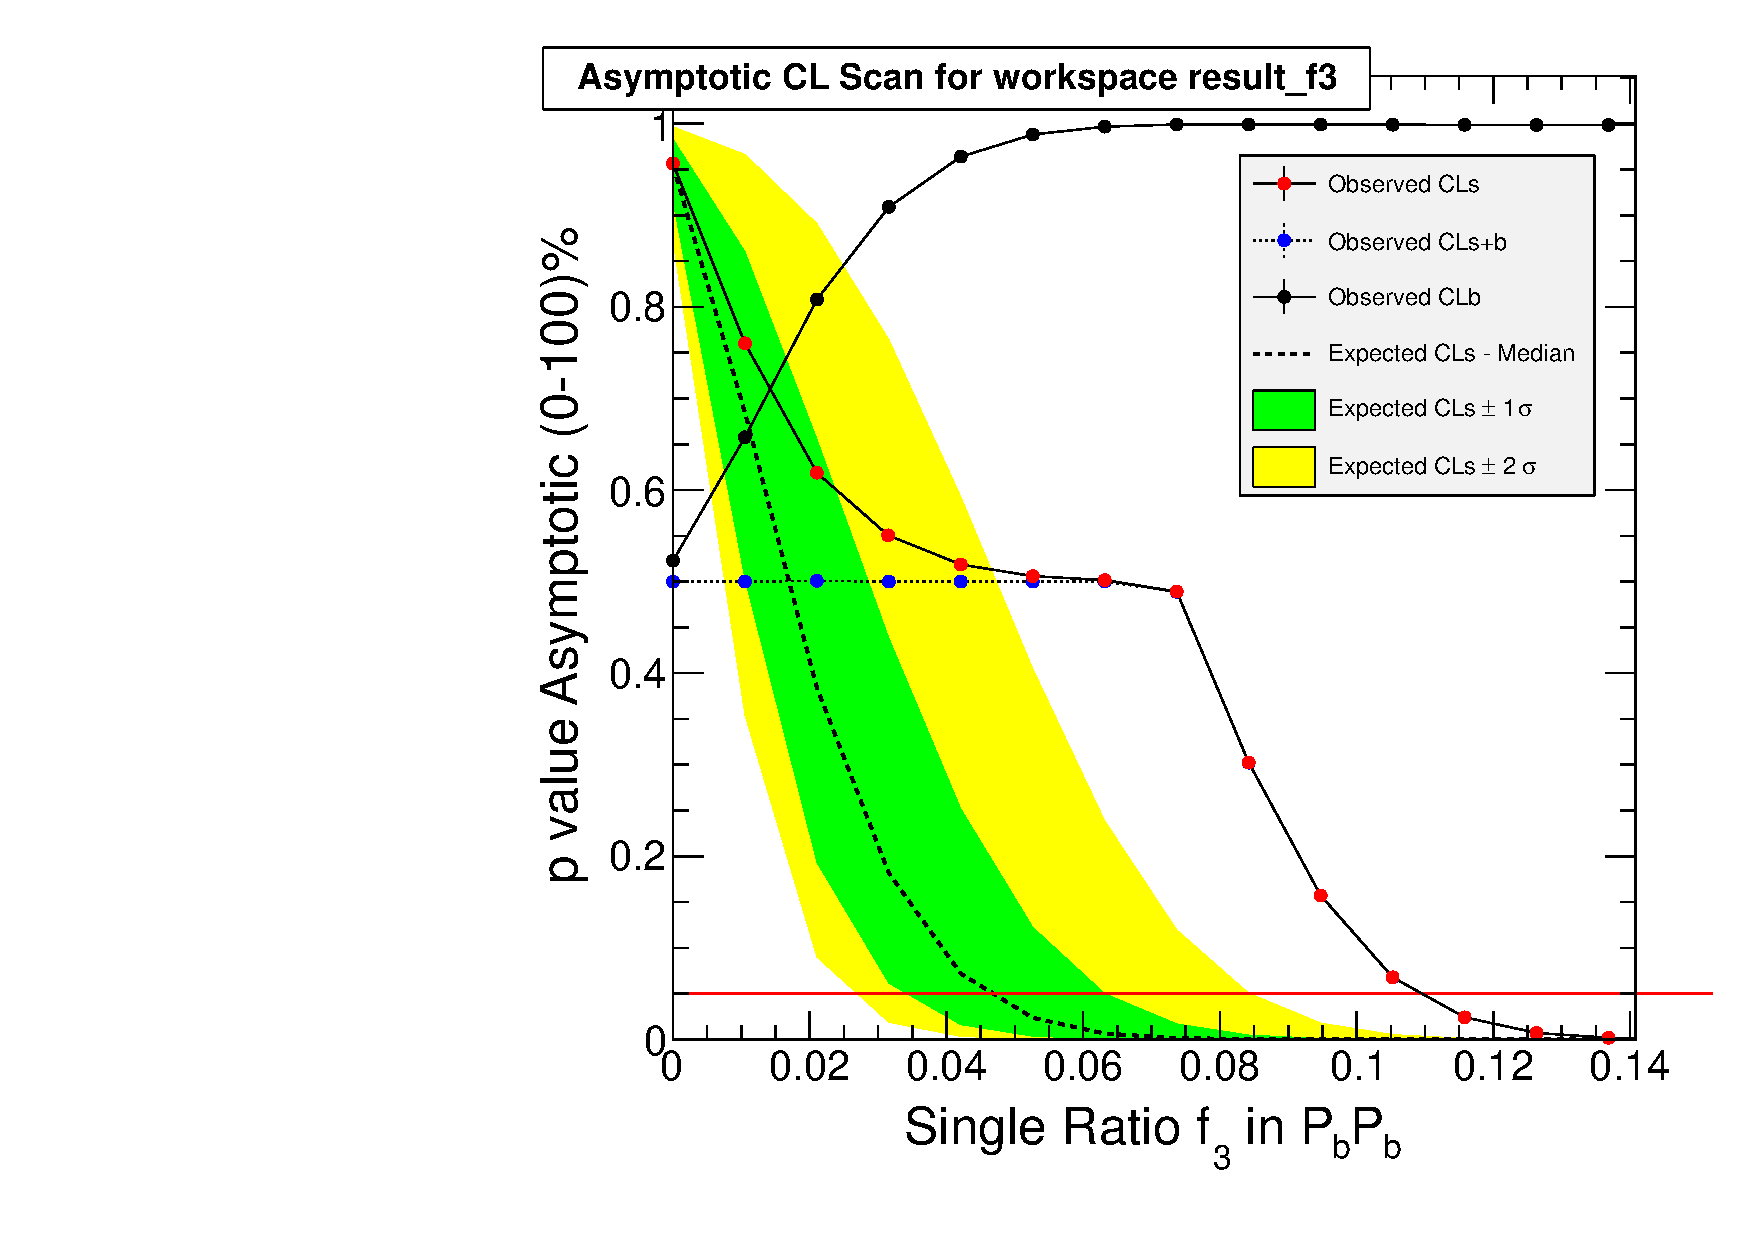
\includegraphics[angle=0,width=0.4\textwidth]{figures/limits/Asymptotic_0100}\label{fig:Asmp_0100}}\\
    \subfigure[Bayesian posterior]{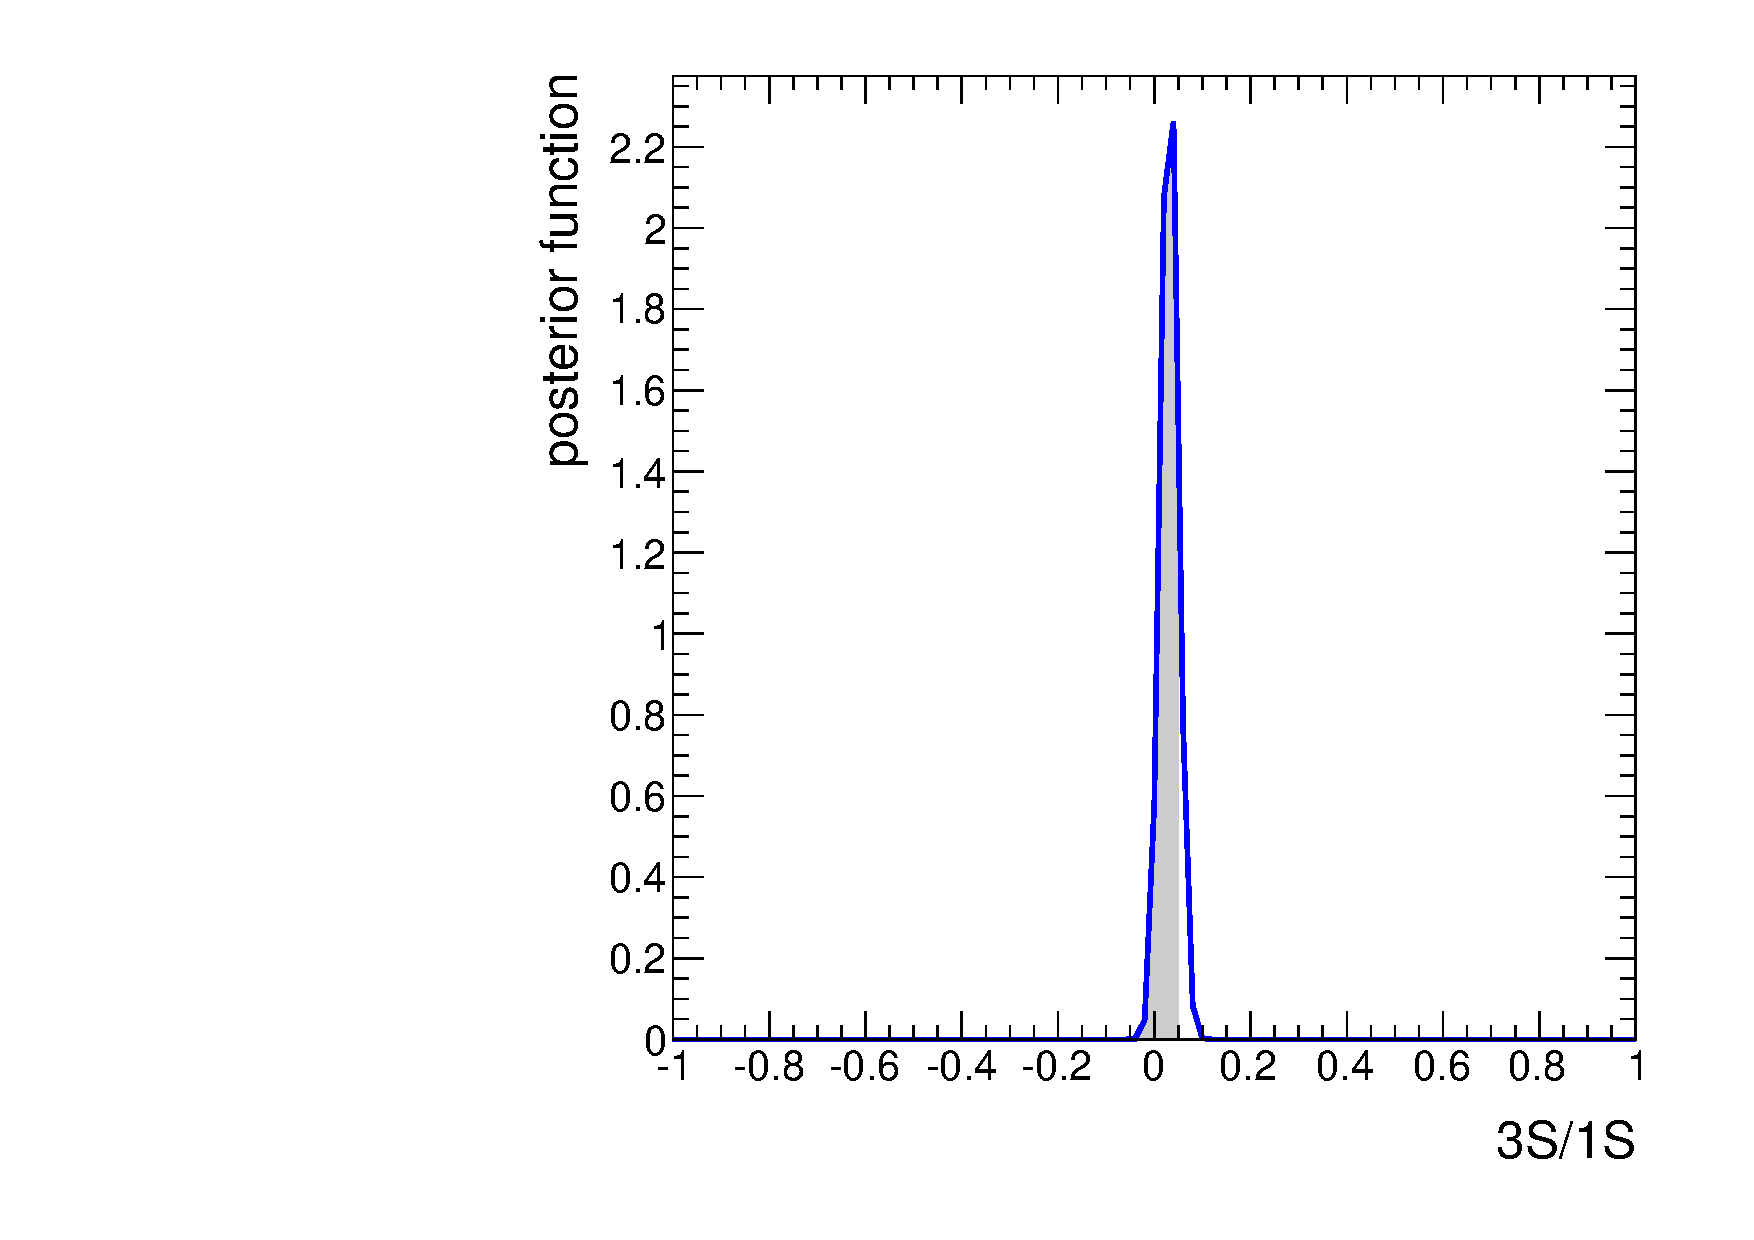
\includegraphics[angle=0,width=0.5\textwidth]{figures/limits/bayesian_num_posterior_0100}\label{fig:bayesian_post_0100}}
    \subfigure[Markov Chain Montecarlo]{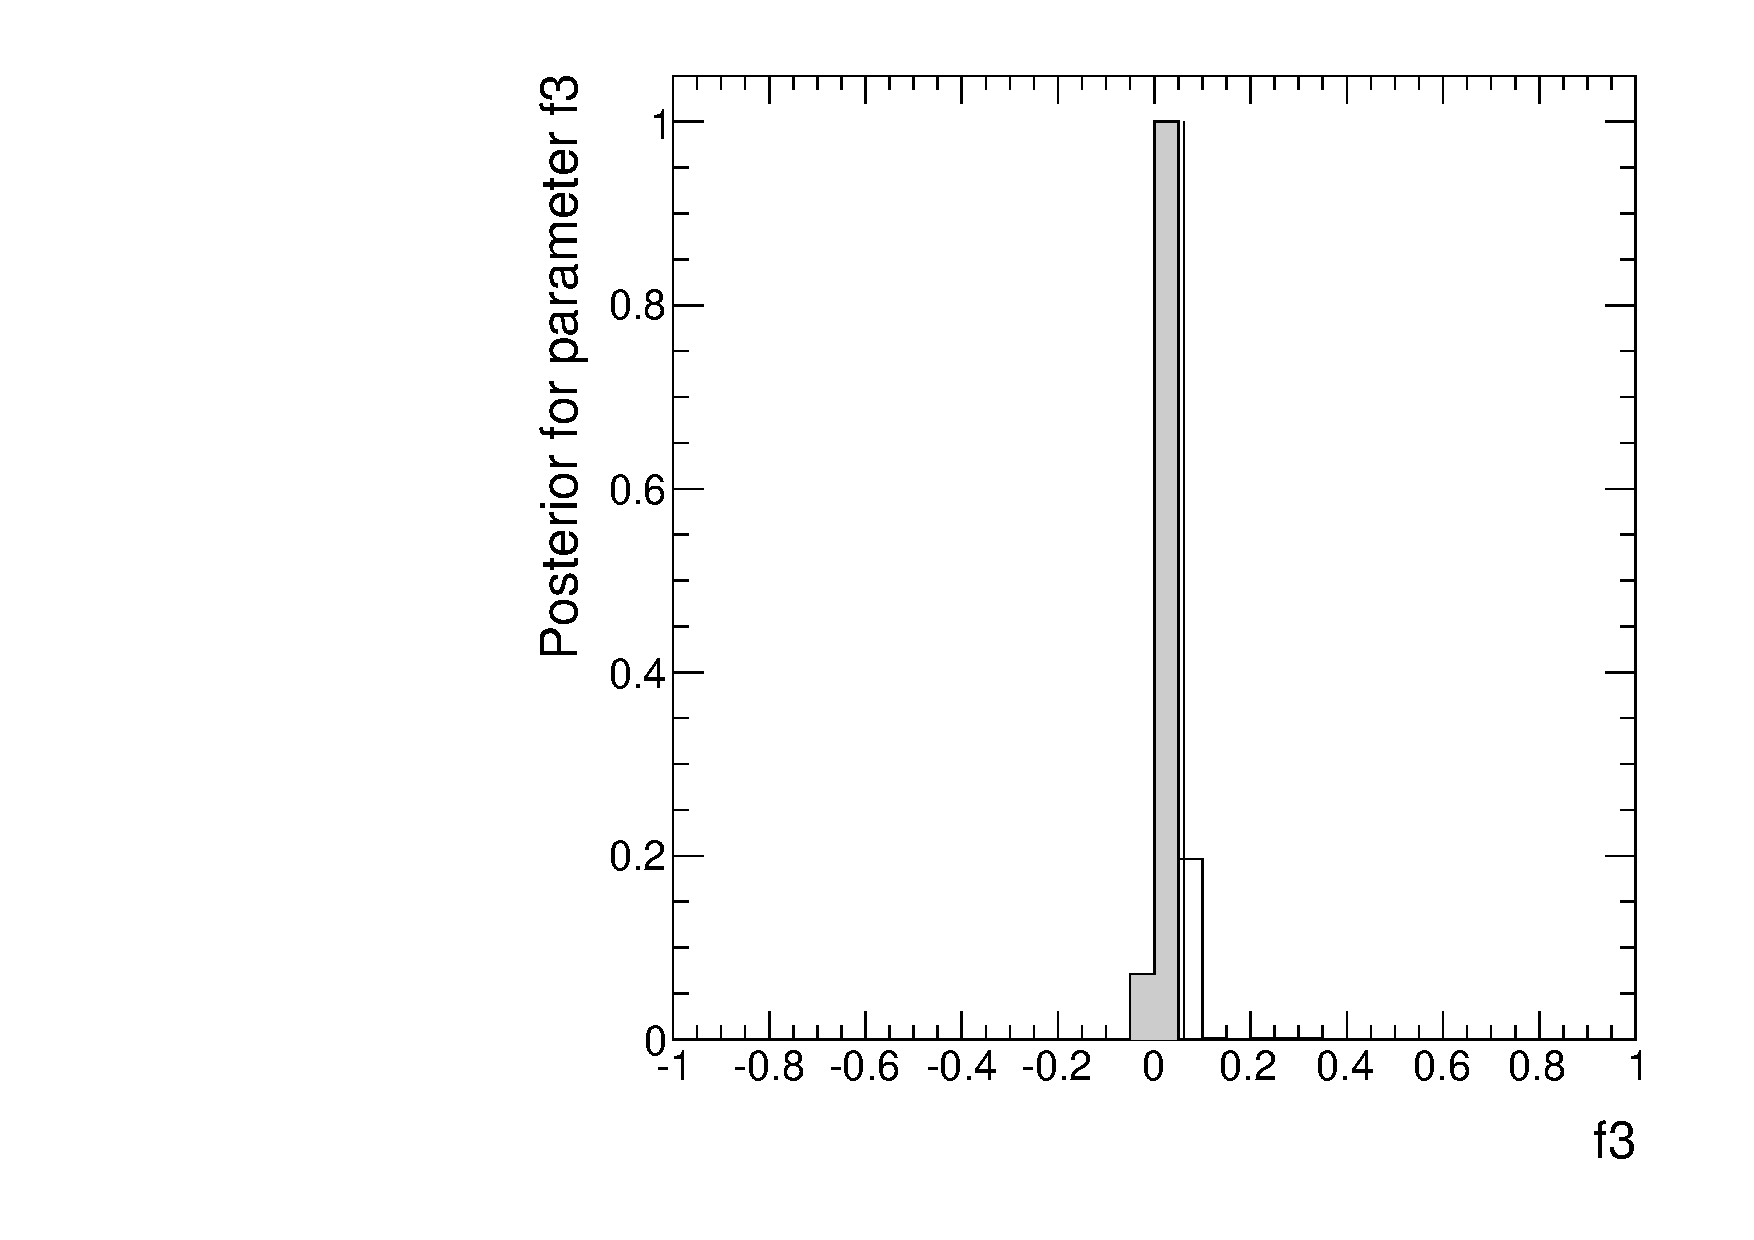
\includegraphics[angle=0,width=0.5\textwidth]{figures/limits/bayesian_mcmc_posterior_0100}\label{fig:bayesian_mcmc_0100}}
    \caption{CLs and Bayesian cross checks for the centrality integrated bin, using uniform prior. Figs~\ref{fig:CLs_0100},~\ref{fig:Asmp_0100}: p-value Scan with different test statistics using 1000 pseudo experiments at each point; Figs~\ref{fig:bayesian_post_0100},~\ref{fig:bayesian_mcmc_0100}: Two different Bayesian approaches: Numerical calculation and Markov Chain Monte Carlo. \emph{(Note: being updated)}}
    \label{fig:limits_xchecks}
  \end{center}
\end{figure}



\begin{figure}[hbtp]
  \begin{center}
    \subfigure[Bayesian posterior]{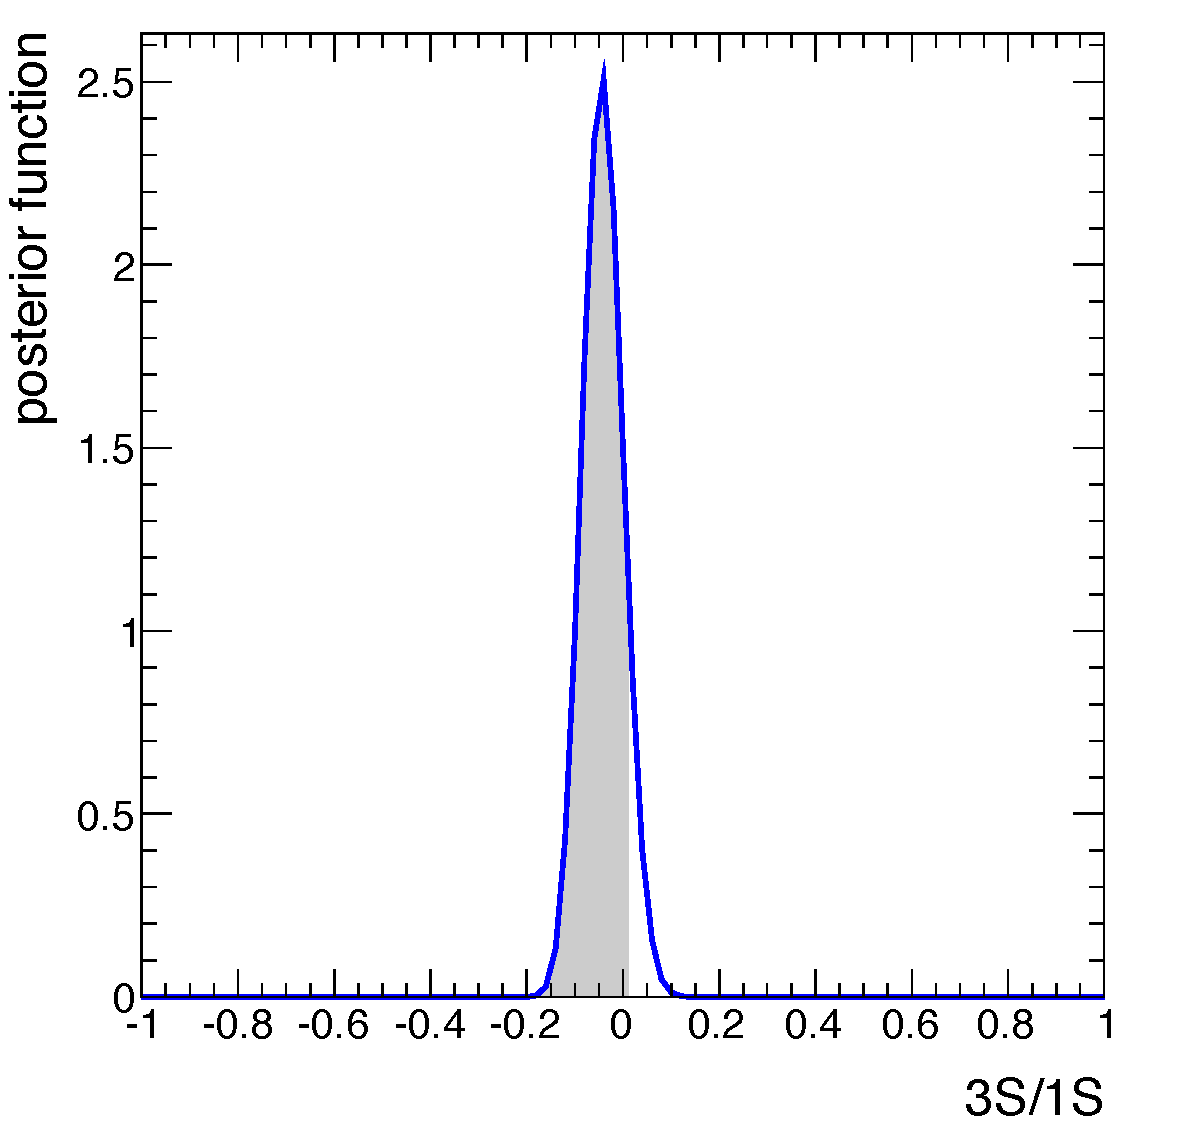
\includegraphics[angle=0,width=0.5\textwidth]{figures/limits/bayesian_num_posterior_3040}\label{fig:bayesian_post_3040}}
%   \subfigure[Markov Chain MonteCarlo steps]{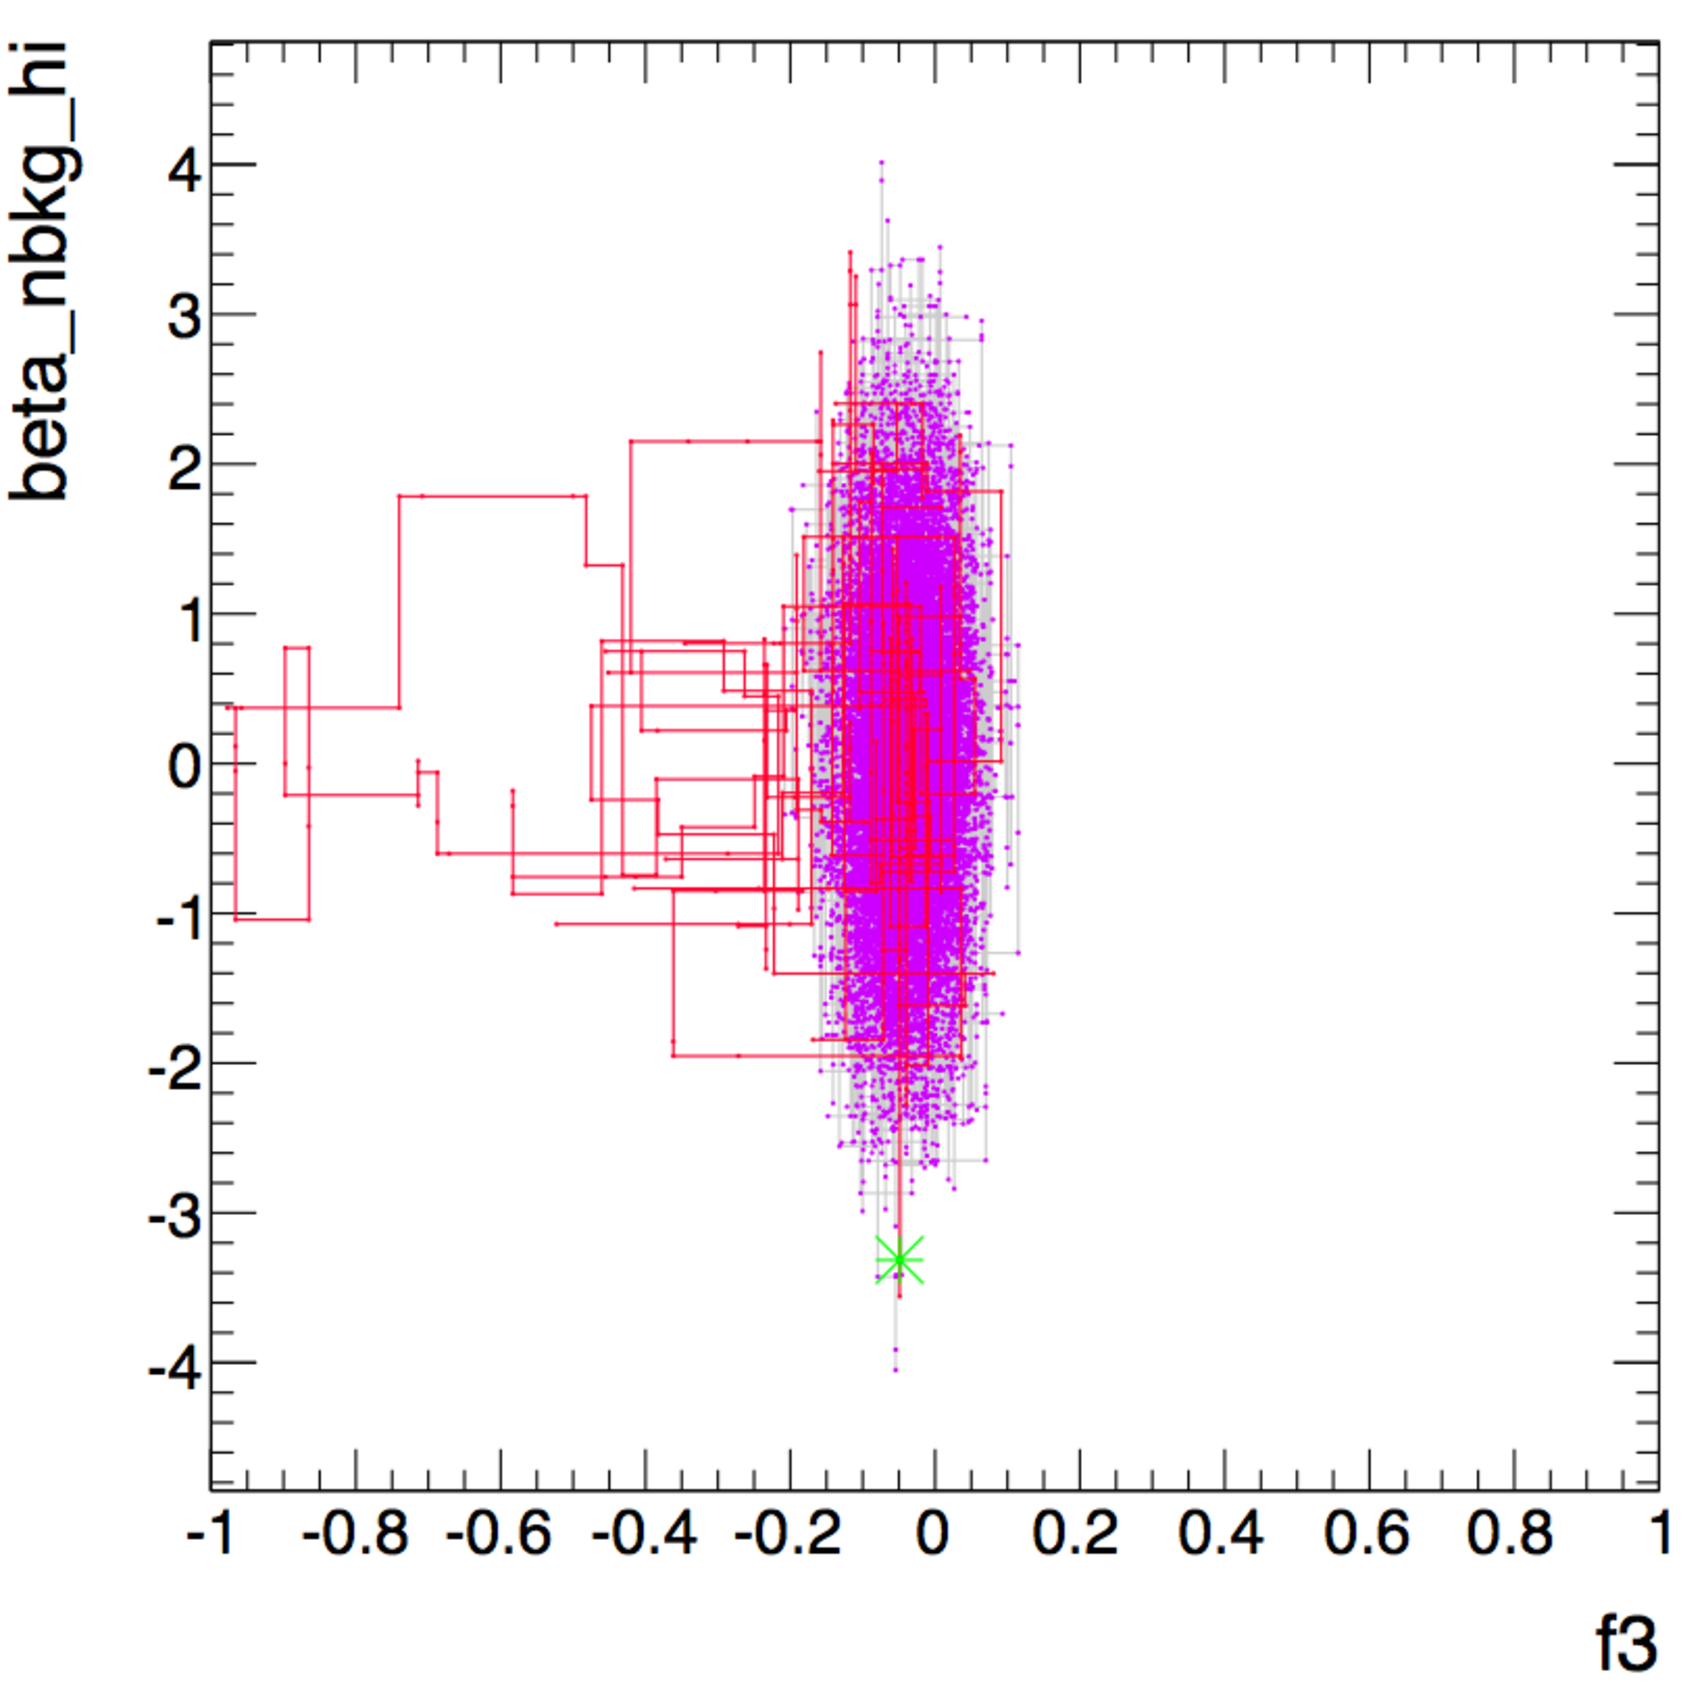
\includegraphics[angle=0,width=0.5\textwidth]{figures/limits/scatter_mcmc_f3_vs_beta_nbkg_3040_lores}\label{fig:scatter_mcmc}} 
    \subfigure[MC Markov Chain posterior]{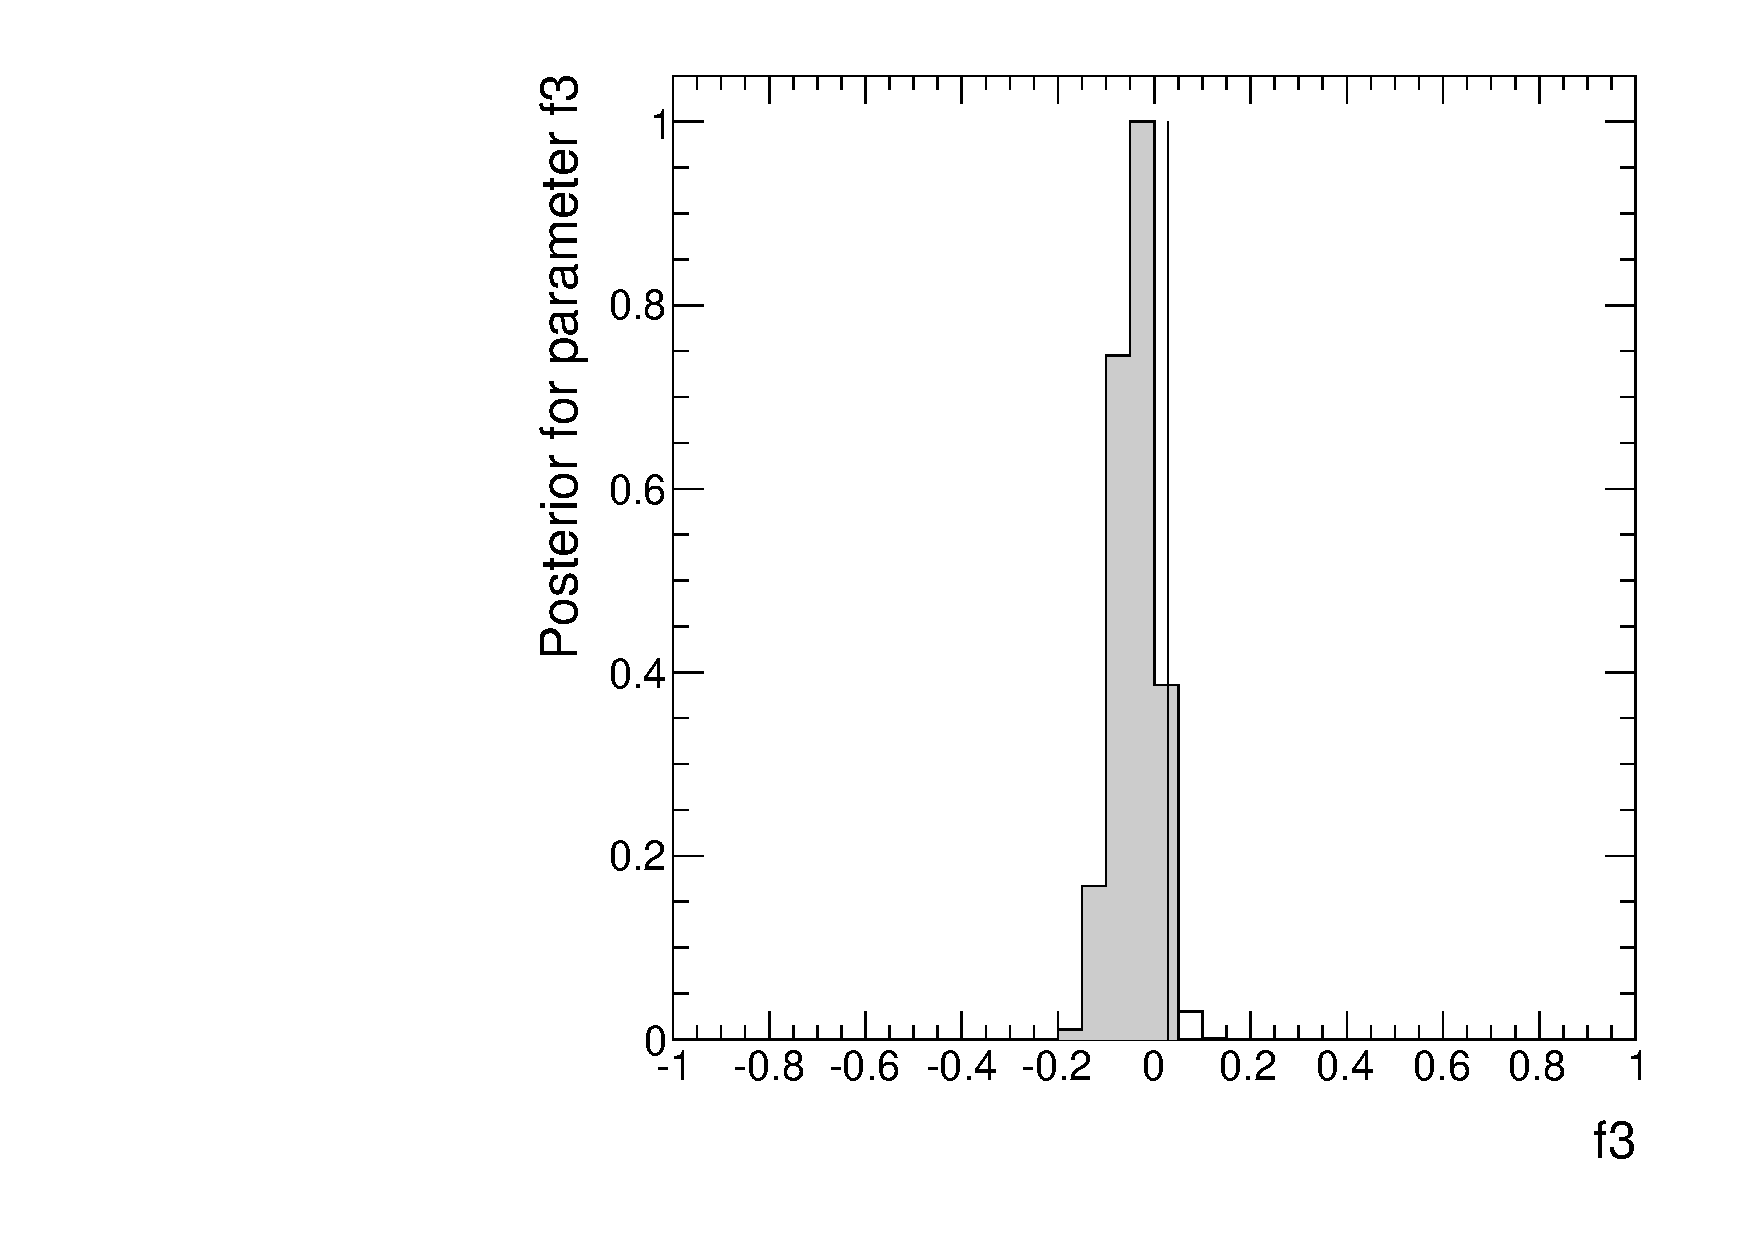
\includegraphics[angle=0,width=0.5\textwidth]{figures/limits/bayesian_mcmc_posterior_3040}\label{fig:bayesian_mcmc_3040}}
    \caption{Bayesian results for 40-50\% centrality bin. Figures~\ref{fig:bayesian_post_3040},~\ref{fig:bayesian_mcmc_3040}: Bayesian Numeric Calculator and Montecarlo Markov Chain. % ; Figs~\ref{fig:scatter_mcmc}: Number of steps in chain: 26701.
\emph{(Note: being updated)}
}
    \label{fig:bayesian}
  \end{center}
\end{figure}

%\begin{figure}[hbtp]
%  \begin{center}
%    \subfigure[Pseudo Experiments for null and alternative hypotheses and test statistics]{\includegraphics[angle=0,width=1.0\textwidth]{figures/limits/FC_toys_0100}\label{fig:FC_toys_0100}}\\
%    \caption{A thousand pseudo experiments for each of the ten points scanned. Figs~\ref{fig:FC_toys_0100}:$ H_{sb}$; red curve, $H_{b}$ blue curve and black line is our Test Statistics}
%    \label{fig:toys}
%  \end{center}
%\end{figure}


 
\begin{table}[!v]
  \centering
  \caption{Single-ratio upper limits. \emph{(Note: being updated)}}
  \begin{tabular}{c|c|c|c|c}
    \hline
    & $R_{3} $ & Feldman-Cousins & frequentist scan $CL_{s}$ & asymptotic scan \\
    \hline
    0 - 5\%   & $0.043 \pm 0.051$ & $ 0.147 \pm 0.003$ & $0.143 \pm 0.005$ & $0.129$ \\
    5 - 10\% & $0.018 \pm 0.055$ & $0.1368 \pm 0.0009$ & $0.2222 \pm 0.0002$ & $0.124$ \\
    10 - 20\% & $0.0062 \pm  0.0352$ & $0.1390 \pm 0.0009$ & $0.3129 \pm 0.0005$ & $0.074$ \\
    20 - 30\% & $0.052 \pm 0.036$ & $0.1232 \pm 0.0006 $ & $0.110 \pm 0.0003$ & $0.11$ \\
    30 - 40\% & $-0.046 \pm 0.045$ & $0.0407 \pm 0.0001$ & $0.065 \pm 0.011$ & $0.063$ \\
    40 - 50\% & $0.23 \pm 0.070$ &$ 0.0980 \pm 0.0003$ & $0.364 \pm 0.003$ & $0.35$\\
    50 - 100\% & $ -0.069 \pm 0.061 $ & $0.054 \pm 0.0002$ & $0.081 \pm 0.005 $ & $0.084$\\
    \hline
    0 - 100\% & $0.032 \pm 0.019$ & $0.0695 \pm 0.0004$ & $0.0638 \pm 0.00006$ & $0.0631$\\
    \hline
  \end{tabular}
  \label{tab:upperlimits}
\end{table}

\begin{table}[!v]
  \centering
  \caption{Single-ratio credible intervals: Bayesian cross checks. \emph{(Note: being updated)}}
  \begin{tabular}{c|c|c|c}
    \hline
    & $R{3} $ & Bayesian calculator & $MCMC$  \\
    \hline
    0 - 5\%   & $0.043 \pm 0.051$ & $[-1, 0.12]$ & $[-1, 0.14]$\\
    5 - 10\% & $0.018 \pm 0.055$  & $[-1, 0.091]$ & $ [-1, 0.47]$\\
    10 - 20\% & $0.0062 \pm  0.0352$  & $[-1, 0.051]$ & $[-1, 0.070]$\\
    20 - 30\% & $0.052 \pm 0.036$ & $[-1, 0.091]$ & $[-1, 0.11]$\\
    30 - 40\% & $-0.046 \pm 0.045$ & $[-1, 0.010]$ & $[-1, 0.028]$\\
    40 - 50\% & $0.23 \pm 0.070$ & $[-1, 0.33]$ & $[-1, 0.41]$\\
    50 - 100\% & $ -0.069 \pm 0.061 $ & $ [-1, 0.010]$ & $[-1, 0.062]$  \\
    \hline    
    0 - 100\% & $0.032 \pm 0.019$& $[-1, 0.051]$ & $[-1, 0.062]$\\
    \hline
  \end{tabular}
  \label{tab:credible_intervals}
\end{table}

\end{chapter}